\documentclass[aspectratio=169,10pt]{beamer}

% Shared Beamer setup for Fall 2026 course slides.
% Clean Cal Poly-inspired theme: no custom class files or uncommon packages.
\mode<presentation>{
  \usetheme{default}
  \usefonttheme{professionalfonts}
}

\definecolor{CalPolyGreen}{HTML}{154734}
\definecolor{CalPolyGold}{HTML}{BD8B13}
\definecolor{CalPolySage}{HTML}{7FA28F}
\definecolor{CalPolyMint}{HTML}{DDF1E7}
\definecolor{CalPolySand}{HTML}{A29F86}
\definecolor{CalPolyBeige}{HTML}{EFEEDE}
\definecolor{DeckInk}{HTML}{1F2933}
\definecolor{DeckMuted}{HTML}{5F6B7A}
\definecolor{DeckSoft}{HTML}{F7F7F5}

\setbeamersize{text margin left=0.55in,text margin right=0.55in}
\setbeamercolor{normal text}{fg=DeckInk,bg=white}
\setbeamercolor{structure}{fg=CalPolyGreen}
\setbeamercolor{title}{fg=white}
\setbeamercolor{frametitle}{fg=CalPolyGreen,bg=white}
\setbeamercolor{block title}{bg=CalPolySage,fg=white}
\setbeamercolor{block body}{bg=CalPolyMint,fg=black}
\setbeamercolor{alerted text}{fg=CalPolyGold}

\setbeamerfont{title}{size=\Huge,series=\bfseries}
\setbeamerfont{frametitle}{size=\Large,series=\bfseries}
\setbeamerfont{block title}{size=\normalsize,series=\bfseries}

\setbeamertemplate{navigation symbols}{}
\setbeamertemplate{itemize item}{\color{CalPolyGold}$\blacktriangleright$}
\setbeamertemplate{itemize subitem}{\color{CalPolyGreen}$\bullet$}
\setbeamertemplate{footline}{
  \hfill{\color{DeckMuted}\scriptsize\insertframenumber/\inserttotalframenumber}
  \hspace{0.18in}\vspace{0.12in}
}
\setbeamertemplate{frametitle}{
  \vspace{0.18in}
  \hspace{0.02in}\insertframetitle\par
  \vspace{0.08in}
  \noindent\makebox[\linewidth][l]{%
    {\color{CalPolyGold}\rule{0.55in}{2pt}}%
    {\color{CalPolyGreen}\rule{\dimexpr\linewidth-0.55in\relax}{2pt}}%
  }
}

\newcommand{\CourseNumber}{Course}
\newcommand{\CourseTitle}{Course Title}
\newcommand{\LectureNumber}{0}
\newcommand{\LectureTitle}{Lecture Title}
\newcommand{\LectureDate}{Date}
\newcommand{\CourseUnit}{Unit}

\newcommand{\coursenumber}[1]{\renewcommand{\CourseNumber}{#1}}
\newcommand{\coursetitle}[1]{\renewcommand{\CourseTitle}{#1}}
\newcommand{\lecturenumber}[1]{\renewcommand{\LectureNumber}{#1}}
\newcommand{\lecturetitle}[1]{\renewcommand{\LectureTitle}{#1}}
\newcommand{\lecturedate}[1]{\renewcommand{\LectureDate}{#1}}
\newcommand{\courseunit}[1]{\renewcommand{\CourseUnit}{#1}}

\author{Kirk Duran}
\institute{California Polytechnic State University, San Luis Obispo}
\date{\LectureDate}

\newcommand{\makedecktitle}{
  \begingroup
  \setbeamercolor{background canvas}{bg=CalPolyGreen}
  \begin{frame}[plain]
    \vfill
    \begin{center}
      {\usebeamerfont{title}\color{white}\LectureTitle\par}
      \vspace{0.18in}
      {\Large\color{white}Lecture \LectureNumber\par}
    \end{center}
    \vfill
    \noindent{\color{white}\rule{\linewidth}{1.2pt}}\par
    \vspace{0.08in}
    \noindent\colorbox{CalPolyGold}{\makebox[0.24\linewidth][c]{\color{white}\Large\CourseNumber}}
    \hspace{0.12in}{\color{white}\Large Kirk Duran}
  \end{frame}
  \endgroup
}

\newenvironment{keyidea}{\begin{block}{Key idea}}{\end{block}}
\newenvironment{activity}{\begin{block}{In class}}{\end{block}}
\newenvironment{cpdefinition}{\begin{block}{Definition}}{\end{block}}
\newenvironment{exampleblockcp}{
  \begingroup
  \setbeamercolor{block title}{bg=CalPolySand,fg=white}
  \setbeamercolor{block body}{bg=CalPolyBeige,fg=black}
  \begin{block}{Example}
}{
  \end{block}
  \endgroup
}

\newcommand{\imageplaceholder}[2][0.3in]{%
  \noindent\makebox[\linewidth][c]{%
    \fcolorbox{CalPolySage}{CalPolyBeige}{%
      \parbox[c][#1][c]{0.86\linewidth}{%
        \centering
        {\color{DeckMuted}\scriptsize Image placeholder: }%
        {\color{DeckInk}\scriptsize\ttfamily\detokenize{#2}}%
      }%
    }%
  }%
}

\newcommand{\sectionframe}[1]{
  \begingroup
  \setbeamercolor{background canvas}{bg=CalPolyGreen}
  \begin{frame}[plain]
    \vfill
    {\color{white}\LARGE\bfseries #1\par}
    \vspace{0.18in}
    {\color{CalPolyGold}\rule{0.22\paperwidth}{3pt}}
    {\color{white}\rule{0.62\paperwidth}{3pt}}
    \vfill
  \end{frame}
  \endgroup
}

\newcommand{\placeholdernote}{
  \begin{block}{Placeholder}
    Replace these bullets with the final lecture material, examples, and in-class activities.
  \end{block}
}


\usepackage{tikz}
\usetikzlibrary{arrows.meta,positioning,calc}

\graphicspath{{../assets/lecture-20/}}

% If an image file is not yet available, skip the visual slot.
\newcommand{\lectureimage}[2][1.75in]{%
  \IfFileExists{../assets/lecture-20/#2}{%
    \includegraphics[width=\linewidth,height=#1,keepaspectratio]{#2}%
  }{}%
}

% Explicit placeholder for visuals/examples that will be added later.
\newcommand{\lectureplaceholder}[2][2.35in]{%
  \begin{center}
    \fbox{%
      \begin{minipage}[c][#1][c]{0.90\linewidth}
        \centering
        \small\textit{#2}
      \end{minipage}%
    }
  \end{center}%
}

\setbeamersize{text margin left=0.42in,text margin right=0.42in}

\coursenumber{CS 4880}
\coursetitle{Artificial Intelligence}
\lecturenumber{20}
\lecturetitle{Bayesian Networks II: Sampling and Approximate Inference}
\lecturedate{October 12, 2026}
\courseunit{Probability and Bayesian Networks}

\begin{document}

% Estimated pacing: 50 minutes
% Why approximate inference: 7 min
% Monte Carlo + prior sampling: 9 min
% Rejection sampling: 9 min
% Likelihood weighting: 10 min
% Gibbs sampling: 11 min
% Comparison and synthesis: 4 min

% -----------------------------------------------------------------------------
% Slide 1
% -----------------------------------------------------------------------------
\makedecktitle

\section{When Exact Inference Stops Scaling}

% -----------------------------------------------------------------------------
% Slide 2
% -----------------------------------------------------------------------------
\begin{frame}[shrink=10]{Last Time: Exact Inference Worked}
  For the small robot network,
  \[
    P(O,R,C,L)=P(O)P(R)P(C\mid O,R)P(L\mid O,R),
  \]
  and exact inference gave
  \[
    P(O\mid C=+,L=+)\approx 0.902.
  \]

  \begin{columns}[T,onlytextwidth]
    \begin{column}{0.47\textwidth}
      \begin{block}{What we gained}
        Correctly modeled correlated sensors and obtained an exact posterior.
      \end{block}
    \end{column}
    \begin{column}{0.47\textwidth}
      \begin{block}{What it cost}
        We had to sum over every hidden assignment relevant to the query.
      \end{block}
    \end{column}
  \end{columns}

  \begin{keyidea}
    Exact inference is attractive because it is exact---not because it is always cheap.
  \end{keyidea}
\end{frame}

% -----------------------------------------------------------------------------
% Slide 3
% -----------------------------------------------------------------------------
\begin{frame}[shrink=10]{A Real Robot Network Does Not Stay Small}
  \begin{columns}[T,onlytextwidth]
    \begin{column}{0.54\textwidth}
      Add realistic hidden variables:
      \begin{itemize}
        \item rain, glare, dust, lighting, and surface reflectivity;
        \item pedestrian, bicycle, vehicle, and temporary construction states;
        \item camera, LiDAR, ultrasonic, wheel-slip, and IMU observations;
        \item component health and calibration states.
      \end{itemize}

      Each new variable may introduce new CPTs and new hidden assignments.
    \end{column}
    \begin{column}{0.40\textwidth}
      \lectureimage[3.00in]{slide3.png}
    \end{column}
  \end{columns}

  \begin{keyidea}
    A compact representation can still produce a difficult inference problem.
  \end{keyidea}
\end{frame}

% -----------------------------------------------------------------------------
% Slide 4
% -----------------------------------------------------------------------------
\begin{frame}[shrink=10]{Exact Inference Must Account for Hidden Variables}
  Suppose the query is
  \[
    P(O\mid c,l,u,w),
  \]
  where the robot has four observed sensors but many unobserved environmental variables $H_1,\ldots,H_k$.

  Exact inference requires terms of the form
  \[
    P(O,c,l,u,w)=\sum_{h_1}\cdots\sum_{h_k} P(O,c,l,u,w,h_1,\ldots,h_k).
  \]

  \begin{block}{The problem}
    The graph may be compact, but the number of hidden configurations considered during inference can grow very quickly.
  \end{block}

  \begin{keyidea}
    Representation complexity and inference complexity are related---but they are not the same thing.
  \end{keyidea}
\end{frame}

% -----------------------------------------------------------------------------
% Slide 5
% -----------------------------------------------------------------------------
\begin{frame}[shrink=10]{The Alternative: Estimate Instead of Enumerate}
  What if the robot does not need the exact value
  \[
    P(O\mid e)=0.90231\ldots
  \]
  and would make the same control decision with
  \[
    \widehat{P}(O\mid e)\approx 0.90?
  \]

  \begin{columns}[T,onlytextwidth]
    \begin{column}{0.47\textwidth}
      \begin{block}{Exact inference}
        Deterministically combine factors until the requested probability is computed.
      \end{block}
    \end{column}
    \begin{column}{0.47\textwidth}
      \begin{block}{Approximate inference}
        Generate representative assignments and estimate the requested probability from them.
      \end{block}
    \end{column}
  \end{columns}

  \begin{keyidea}
    Sampling trades deterministic precision for computational tractability.
  \end{keyidea}
\end{frame}

\section{Monte Carlo and Prior Sampling}

% -----------------------------------------------------------------------------
% Slide 6
% -----------------------------------------------------------------------------
\begin{frame}[shrink=10]{A Sample Is One Possible World}
  A complete sample might be
  \[
    O=true,\quad R=false,\quad C=+,\quad L=+.
  \]

  Another might be
  \[
    O=false,\quad R=true,\quad C=+,\quad L=-.
  \]

  If samples are generated according to the Bayesian network, common worlds appear often and unlikely worlds appear rarely.

  \lectureimage[1.55in]{slide6.png}

  \begin{keyidea}
    Sampling turns a probability distribution into a stream of concrete simulated assignments.
  \end{keyidea}
\end{frame}

% -----------------------------------------------------------------------------
% Slide 7
% -----------------------------------------------------------------------------
\begin{frame}[shrink=10]{Monte Carlo Estimation Uses Frequencies}
  To estimate an event $A$, generate $N$ samples and count how often $A$ occurs:
  \[
    \widehat{P}(A)=\frac{N(A)}{N}.
  \]

  Example: in $10{,}000$ samples, suppose $1{,}017$ contain an obstacle.
  \[
    \widehat{P}(O)=\frac{1017}{10000}=0.1017.
  \]

  The true prior in our model is $P(O)=0.10$.

  \begin{keyidea}
    We replace symbolic summation with empirical counting over simulated worlds.
  \end{keyidea}
\end{frame}

% -----------------------------------------------------------------------------
% Slide 8
% -----------------------------------------------------------------------------
\begin{frame}[shrink=10]{More Samples Usually Mean Less Monte Carlo Noise}
  For independent samples, standard Monte Carlo error typically shrinks on the order of
  \[
    \frac{1}{\sqrt{N}}.
  \]

  \begin{center}
  \renewcommand{\arraystretch}{1.3}
  \begin{tabular}{c|c}
    \textbf{Samples} & \textbf{Relative error scale} \\\hline
    $1{,}000$ & $1/\sqrt{1000}$ \\
    $4{,}000$ & about half as large \\
    $100{,}000$ & about one tenth as large as at $1{,}000$
  \end{tabular}
  \end{center}

  \begin{block}{Important tradeoff}
    Ten times more accuracy does not usually require ten times more samples---it can require roughly one hundred times more.
  \end{block}

  \begin{keyidea}
    Approximate inference gives us a knob: spend more computation to reduce statistical error.
  \end{keyidea}
\end{frame}

% -----------------------------------------------------------------------------
% Slide 9
% -----------------------------------------------------------------------------
\begin{frame}[shrink=10]{Prior Sampling Follows the Graph}
  Generate variables in topological order.

  For the robot network:
  \begin{enumerate}
    \item Sample $O\sim P(O)$.
    \item Sample $R\sim P(R)$.
    \item Sample $C\sim P(C\mid O,R)$.
    \item Sample $L\sim P(L\mid O,R)$.
  \end{enumerate}

  \begin{center}
  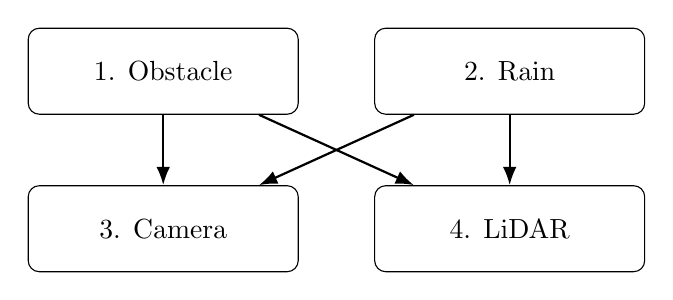
\begin{tikzpicture}[>=Latex,every node/.style={draw,rounded corners,align=center,minimum width=1.35in,minimum height=0.43in}]
    \node (o) at (-2.2,1.0) {1. Obstacle};
    \node (r) at ( 2.2,1.0) {2. Rain};
    \node (c) at (-2.2,-1.0) {3. Camera};
    \node (l) at ( 2.2,-1.0) {4. LiDAR};
    \draw[->,thick] (o)--(c);
    \draw[->,thick] (o)--(l);
    \draw[->,thick] (r)--(c);
    \draw[->,thick] (r)--(l);
  \end{tikzpicture}
  \end{center}

  Numbers show one valid topological sampling order; arrows remain the Bayesian-network dependencies.

  \begin{keyidea}
    Each local draw uses only the CPT of that node and the sampled values of its parents.
  \end{keyidea}
\end{frame}

% -----------------------------------------------------------------------------
% Slide 10
% -----------------------------------------------------------------------------
\begin{frame}[shrink=10]{Worked Prior Sample}
  Suppose the random draws produce:
  \[
    O=true \quad \text{because } u_1 < 0.10.
  \]
  \[
    R=false \quad \text{because } u_2 > 0.20.
  \]

  The CPTs now give
  \[
    P(C=+\mid O,\neg R)=0.95,
    \qquad
    P(L=+\mid O,\neg R)=0.98.
  \]

  Two more random draws might therefore produce
  \[
    (O,R,C,L)=(true,false,+,+).
  \]

  \begin{keyidea}
    Prior sampling never constructs the full joint table; the network itself generates samples from the joint distribution.
  \end{keyidea}
\end{frame}

% -----------------------------------------------------------------------------
% Slide 11
% -----------------------------------------------------------------------------
\begin{frame}[shrink=10]{Prior Sampling: Benefits and Pitfalls}
  \begin{columns}[T,onlytextwidth]
    \begin{column}{0.47\textwidth}
      \begin{block}{Benefits}
        \begin{itemize}
          \item simple to implement;
          \item every sample is usable for unconditional queries;
          \item naturally exploits the network factorization;
          \item easy to parallelize.
        \end{itemize}
      \end{block}
    \end{column}
    \begin{column}{0.47\textwidth}
      \begin{block}{Pitfalls}
        \begin{itemize}
          \item does not force observed evidence to occur;
          \item rare events may appear almost never;
          \item conditional queries can waste most samples.
        \end{itemize}
      \end{block}
    \end{column}
  \end{columns}

  \begin{keyidea}
    Prior sampling is excellent for the model's natural distribution and poor when the query conditions on unlikely evidence.
  \end{keyidea}
\end{frame}

\section{Rejection Sampling}

% -----------------------------------------------------------------------------
% Slide 12
% -----------------------------------------------------------------------------
\begin{frame}[shrink=10]{Evidence Changes the Sampling Problem}
  The robot does not usually ask
  \[
    P(O).
  \]
  It asks
  \[
    P(O\mid C=+,L=+).
  \]

  One simple strategy:
  \begin{enumerate}
    \item sample complete worlds from the prior;
    \item reject any world inconsistent with the observed sensor evidence;
    \item estimate the posterior from the remaining worlds.
  \end{enumerate}

  \begin{keyidea}
    Rejection sampling converts prior samples into conditional samples by discarding worlds that contradict the evidence.
  \end{keyidea}
\end{frame}

% -----------------------------------------------------------------------------
% Slide 13
% -----------------------------------------------------------------------------
\begin{frame}[shrink=10]{Rejection Sampling}
  For query variable $X$ and evidence $e$:

  \begin{block}{Algorithm}
    Repeat $N$ times:
    \begin{enumerate}
      \item draw a complete prior sample $s$;
      \item if $s$ disagrees with $e$, discard it;
      \item otherwise increment the count for $X(s)$.
    \end{enumerate}
    Normalize the retained counts.
  \end{block}

  \[
    \widehat{P}(X\mid e)
    =
    \frac{N(X,e)}{N(e)}.
  \]

  \begin{keyidea}
    The method is conceptually clean because accepted samples are distributed according to the desired conditional distribution.
  \end{keyidea}
\end{frame}

% -----------------------------------------------------------------------------
% Slide 14
% -----------------------------------------------------------------------------
\begin{frame}[shrink=10]{Worked Rejection Example}
  Evidence:
  \[
    C=+,\qquad L=+.
  \]

  Imagine $10{,}000$ prior samples:
  \begin{center}
  \renewcommand{\arraystretch}{1.3}
  \begin{tabular}{l|r}
    \textbf{Sample outcome} & \textbf{Count} \\\hline
    agrees with $C=+,L=+$ & $995$ \\
    rejected & $9{,}005$ \\
    accepted and $O=true$ & $898$ \\
    accepted and $O=false$ & $97$
  \end{tabular}
  \end{center}

  Then
  \[
    \widehat{P}(O\mid c,l)=\frac{898}{995}\approx 0.903.
  \]

  \begin{keyidea}
    The estimate is close to the exact $0.902$ result---but more than $90\%$ of the simulation work was discarded.
  \end{keyidea}
\end{frame}

% -----------------------------------------------------------------------------
% Slide 15
% -----------------------------------------------------------------------------
\begin{frame}[shrink=10]{Rare Evidence Can Destroy Rejection Sampling}
  If the probability of the evidence is
  \[
    P(e)=0.001,
  \]
  then only about one sample in one thousand is expected to survive.

  To obtain roughly $1{,}000$ accepted samples, we may need around
  \[
    1{,}000{,}000
  \]
  prior samples.

  \lectureimage[1.55in]{slide15.png}

  \begin{keyidea}
    Rejection sampling spends computation generating exactly the worlds we already know did not happen.
  \end{keyidea}
\end{frame}

% -----------------------------------------------------------------------------
% Slide 16
% -----------------------------------------------------------------------------
\begin{frame}[shrink=10]{Rejection Sampling: Benefits and Pitfalls}
  \begin{columns}[T,onlytextwidth]
    \begin{column}{0.47\textwidth}
      \begin{block}{Benefits}
        \begin{itemize}
          \item extremely simple;
          \item accepted samples have equal weight;
          \item easy to reason about and debug;
          \item good when evidence is common.
        \end{itemize}
      \end{block}
    \end{column}
    \begin{column}{0.47\textwidth}
      \begin{block}{Pitfalls}
        \begin{itemize}
          \item acceptance rate is approximately $P(e)$;
          \item rare evidence wastes almost all samples;
          \item high-dimensional evidence can make acceptance collapse.
        \end{itemize}
      \end{block}
    \end{column}
  \end{columns}

  \begin{keyidea}
    Rejection sampling is not bad because it is approximate; it is bad when the conditioning event is hard to observe by chance.
  \end{keyidea}
\end{frame}

\section{Likelihood Weighting}

% -----------------------------------------------------------------------------
% Slide 17
% -----------------------------------------------------------------------------
\begin{frame}[shrink=10]{Can We Stop Throwing Evidence Away?}
  We already know
  \[
    C=+,\qquad L=+.
  \]

  So likelihood weighting does not sample those variables at all.

  Instead:
  \begin{itemize}
    \item lock evidence variables to their observed values;
    \item sample only the non-evidence variables;
    \item attach a weight measuring how compatible the sampled world is with the evidence.
  \end{itemize}

  \begin{keyidea}
    Likelihood weighting forces every sample to respect the evidence, then compensates statistically with a weight.
  \end{keyidea}
\end{frame}

% -----------------------------------------------------------------------------
% Slide 18
% -----------------------------------------------------------------------------
\begin{frame}[shrink=10]{Likelihood Weighting Algorithm}
  Start each sample with weight
  \[
    w=1.
  \]

  Traverse variables in topological order:
  \begin{itemize}
    \item if $X_i$ is not evidence, sample it from $P(X_i\mid Parents(X_i))$;
    \item if $X_i=e_i$ is evidence, keep $e_i$ fixed and update
  \end{itemize}

  \[
    w \leftarrow w\,P(e_i\mid Parents(E_i)).
  \]

  Therefore
  \[
    w=\prod_{E_i\in e}P(e_i\mid Parents(E_i)).
  \]

  \begin{keyidea}
    Samples that make the observed evidence plausible contribute more to the estimate.
  \end{keyidea}
\end{frame}

% -----------------------------------------------------------------------------
% Slide 19
% -----------------------------------------------------------------------------
\begin{frame}[shrink=10]{Worked Weight: Obstacle, No Rain}
  Evidence is fixed:
  \[
    C=+,\qquad L=+.
  \]

  Suppose we sample
  \[
    O=true,\qquad R=false.
  \]

  Then
  \[
    w=P(C=+\mid O,\neg R)P(L=+\mid O,\neg R)
  \]
  \[
    =(0.95)(0.98)=0.931.
  \]

  This sample contributes weight $0.931$ to the $O=true$ bucket.

  \begin{keyidea}
    We never reject this sample; its influence is proportional to how well it explains the observed sensors.
  \end{keyidea}
\end{frame}

% -----------------------------------------------------------------------------
% Slide 20
% -----------------------------------------------------------------------------
\begin{frame}[shrink=10]{A Weak Explanation Gets a Small Weight}
  Suppose instead we sample
  \[
    O=false,\qquad R=false.
  \]

  The evidence likelihood is
  \[
    w=(0.05)(0.02)=0.001.
  \]

  Compare:
  \[
    \frac{0.931}{0.001}=931.
  \]

  The first world contributes $931$ times as much weight to the posterior estimate.

  \begin{keyidea}
    Likelihood weighting preserves unlikely samples without pretending that they explain the evidence well.
  \end{keyidea}
\end{frame}

% -----------------------------------------------------------------------------
% Slide 21
% -----------------------------------------------------------------------------
\begin{frame}[shrink=10]{Weighted Counts Produce the Posterior}
  After many samples, accumulate weights instead of raw counts.

  Example:
  \begin{center}
  \renewcommand{\arraystretch}{1.3}
  \begin{tabular}{c|r}
    \textbf{Query value} & \textbf{Total accumulated weight} \\\hline
    $O=true$ & $89.9$ \\
    $O=false$ & $9.8$
  \end{tabular}
  \end{center}

  Normalize:
  \[
    \widehat{P}(O\mid c,l)
    =
    \frac{89.9}{89.9+9.8}
    \approx 0.902.
  \]

  \begin{keyidea}
    The weights replace rejection: every sample participates, but not every sample participates equally.
  \end{keyidea}
\end{frame}

% -----------------------------------------------------------------------------
% Slide 22
% -----------------------------------------------------------------------------
\begin{frame}[shrink=10]{Pitfall: Weight Degeneracy}
  For many evidence variables,
  \[
    w=\prod_i P(e_i\mid Parents(E_i)).
  \]

  Products of many probabilities can make most weights extremely small while a few samples dominate.

  A useful diagnostic is the effective sample size
  \[
    ESS\approx \frac{(\sum_i w_i)^2}{\sum_i w_i^2}.
  \]

  \begin{block}{Example}
    We may generate $10{,}000$ weighted samples but obtain an ESS of only a few hundred because nearly all useful weight sits on a small subset.
  \end{block}

  \begin{keyidea}
    Keeping every sample is not the same as getting useful information from every sample.
  \end{keyidea}
\end{frame}

% -----------------------------------------------------------------------------
% Slide 23
% -----------------------------------------------------------------------------
\begin{frame}[shrink=10]{Likelihood Weighting: Benefits and Pitfalls}
  \begin{columns}[T,onlytextwidth]
    \begin{column}{0.47\textwidth}
      \begin{block}{Benefits}
        \begin{itemize}
          \item never rejects evidence-inconsistent samples;
          \item often much better than rejection for rare evidence;
          \item simple extension of ancestral sampling;
          \item easy to parallelize.
        \end{itemize}
      \end{block}
    \end{column}
    \begin{column}{0.47\textwidth}
      \begin{block}{Pitfalls}
        \begin{itemize}
          \item weights can become highly unequal;
          \item evidence far downstream may be hard to explain;
          \item effective sample size can be far below sample count.
        \end{itemize}
      \end{block}
    \end{column}
  \end{columns}

  \begin{keyidea}
    Likelihood weighting fixes wasted rejection but can replace it with a different failure mode: concentrated weights.
  \end{keyidea}
\end{frame}

\section{Gibbs Sampling}

% -----------------------------------------------------------------------------
% Slide 24
% -----------------------------------------------------------------------------
\begin{frame}[shrink=10]{A Different Strategy: Walk Through Possible Worlds}
  Prior, rejection, and likelihood weighting repeatedly build a world from scratch.

  Gibbs sampling instead:
  \begin{enumerate}
    \item fixes the evidence variables;
    \item starts with any assignment to the remaining variables;
    \item repeatedly resamples one non-evidence variable conditioned on the current values of the others.
  \end{enumerate}

  The result is a \textbf{Markov chain} of related assignments.

  \lectureimage[1.45in]{slide24.png}

  \begin{keyidea}
    Gibbs sampling explores the posterior directly rather than hoping prior samples happen to match the evidence.
  \end{keyidea}
\end{frame}

% -----------------------------------------------------------------------------
% Slide 25
% -----------------------------------------------------------------------------
\begin{frame}[shrink=10]{Only the Markov Blanket Is Needed}
  To resample a variable $X$, Gibbs sampling needs only its \textbf{Markov blanket}:
  \begin{itemize}
    \item parents of $X$;
    \item children of $X$;
    \item other parents of those children.
  \end{itemize}

  For obstacle $O$ in our robot network:
  \[
    MB(O)=\{C,L,R\}.
  \]

  \begin{center}
  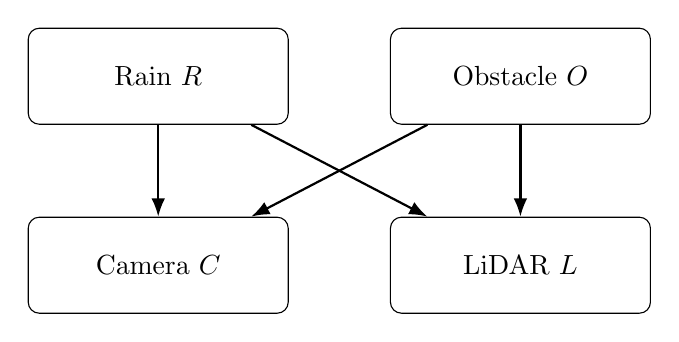
\begin{tikzpicture}[>=Latex,every node/.style={draw,rounded corners,align=center,minimum width=1.3in,minimum height=0.48in}]
    \node (r) at (0,1.2) {Rain $R$};
    \node (o) at (4.6,1.2) {Obstacle $O$};
    \node (c) at (0,-1.2) {Camera $C$};
    \node (l) at (4.6,-1.2) {LiDAR $L$};
    \draw[->,thick] (r)--(c); \draw[->,thick] (r)--(l);
    \draw[->,thick] (o)--(c); \draw[->,thick] (o)--(l);
  \end{tikzpicture}
  \end{center}

  \begin{keyidea}
    Local graph structure makes each Gibbs update cheaper than recomputing the entire joint distribution.
  \end{keyidea}
\end{frame}

% -----------------------------------------------------------------------------
% Slide 26
% -----------------------------------------------------------------------------
\begin{frame}[shrink=10]{Worked Gibbs Update: Resample the Obstacle}
  Keep evidence fixed:
  \[
    C=+,\qquad L=+.
  \]
  Suppose the current state has $R=true$.

  Score the two possible obstacle states:
  \[
    O=true:\quad (0.10)(0.85)(0.90)=0.0765,
  \]
  \[
    O=false:\quad (0.90)(0.25)(0.20)=0.045.
  \]

  Normalize:
  \[
    P(O=true\mid R=true,c,l)
    =\frac{0.0765}{0.0765+0.045}
    \approx 0.630.
  \]

  \begin{keyidea}
    One Gibbs update draws a new value from the variable's conditional distribution given its current neighborhood.
  \end{keyidea}
\end{frame}

% -----------------------------------------------------------------------------
% Slide 27
% -----------------------------------------------------------------------------
\begin{frame}[shrink=10]{Then Resample Another Hidden Variable}
  Suppose the chain currently has $O=true$.

  For rain:
  \[
    R=true:\quad (0.20)(0.85)(0.90)=0.153,
  \]
  \[
    R=false:\quad (0.80)(0.95)(0.98)=0.7448.
  \]

  Therefore
  \[
    P(R=true\mid O=true,c,l)
    =\frac{0.153}{0.153+0.7448}
    \approx 0.170.
  \]

  Alternate updates to $O$, $R$, and any other hidden variables; record their visited states.

  \begin{keyidea}
    The chain gradually spends time in assignments in proportion to their posterior probability.
  \end{keyidea}
\end{frame}

% -----------------------------------------------------------------------------
% Slide 28
% -----------------------------------------------------------------------------
\begin{frame}[shrink=10]{Gibbs Has Different Failure Modes}
  \begin{columns}[T,onlytextwidth]
    \begin{column}{0.31\textwidth}
      \begin{block}{Burn-in}
        Early samples can reflect the arbitrary starting state more than the target posterior.
      \end{block}
    \end{column}
    \begin{column}{0.31\textwidth}
      \begin{block}{Autocorrelation}
        Consecutive samples are related, so $N$ Gibbs samples contain less information than $N$ independent samples.
      \end{block}
    \end{column}
    \begin{column}{0.31\textwidth}
      \begin{block}{Slow mixing}
        Strong dependencies can trap the chain in one region of state space for a long time.
      \end{block}
    \end{column}
  \end{columns}

  \lectureimage[1.35in]{slide28.png}

  \begin{keyidea}
    Gibbs avoids rejection and weight collapse, but the price is dependence between samples and uncertain convergence speed.
  \end{keyidea}
\end{frame}

\section{Choosing an Approximate Inference Method}

% -----------------------------------------------------------------------------
% Slide 29
% -----------------------------------------------------------------------------
\begin{frame}[shrink=10]{Same Goal, Different Failure Modes}
  \begin{center}
  \renewcommand{\arraystretch}{1.28}
  \begin{tabular}{l|p{0.25\textwidth}|p{0.32\textwidth}}
    \textbf{Method} & \textbf{Best feature} & \textbf{Main failure mode} \\\hline
    Prior sampling & simplest; all samples usable for priors & poor conditional inference for rare evidence \\
    Rejection sampling & accepted samples are easy to interpret & acceptance collapses as $P(e)$ becomes small \\
    Likelihood weighting & forces evidence; parallelizable & weight degeneracy / low ESS \\
    Gibbs sampling & explores posterior directly & burn-in, autocorrelation, slow mixing
  \end{tabular}
  \end{center}

  \begin{keyidea}
    There is no universally best sampler; each method moves the computational difficulty somewhere different.
  \end{keyidea}
\end{frame}

% -----------------------------------------------------------------------------
% Slide 30
% -----------------------------------------------------------------------------
\begin{frame}[shrink=10]{Takeaways: Approximation Is an Engineering Decision}
  \begin{itemize}
    \item Exact inference gives a deterministic answer but can become computationally expensive.
    \item Prior sampling estimates probabilities from worlds generated by the Bayesian network.
    \item Rejection sampling conditions by discarding samples that disagree with evidence.
    \item Likelihood weighting fixes evidence and assigns each sample an evidence likelihood weight.
    \item Gibbs sampling forms a Markov chain by repeatedly resampling non-evidence variables from local conditional distributions.
    \item Sample count alone is not enough: acceptance rate, weight concentration, and mixing determine how much information the computation actually produced.
  \end{itemize}

  \begin{keyidea}
    Approximate inference is not ``less rigorous'' inference: it explicitly trades exactness for runtime and measures the consequences of that trade.
  \end{keyidea}
\end{frame}

\end{document}
